 
\documentclass[../main.tex]{subfiles}

\begin{document}

\subsection*{System Architecture}

The LeafAI query engine was designed using a modular, micro service-based architecture with a central API (Application Program Interface) which orchestrates end-to-end query generation. Inter-module communication is performed using gRPC \cite{grpc}, a robust open-source remote procedure call framework which enables language-agnostic service integration. This allows individual modules to be implemented (and substituted) in programming languages and using libraries well-suited to a given task. A diagram of the LeafAI query engine architecture is shown in Figure \ref{fig_leafai_architecture}. 

\begin{figure}[h]
  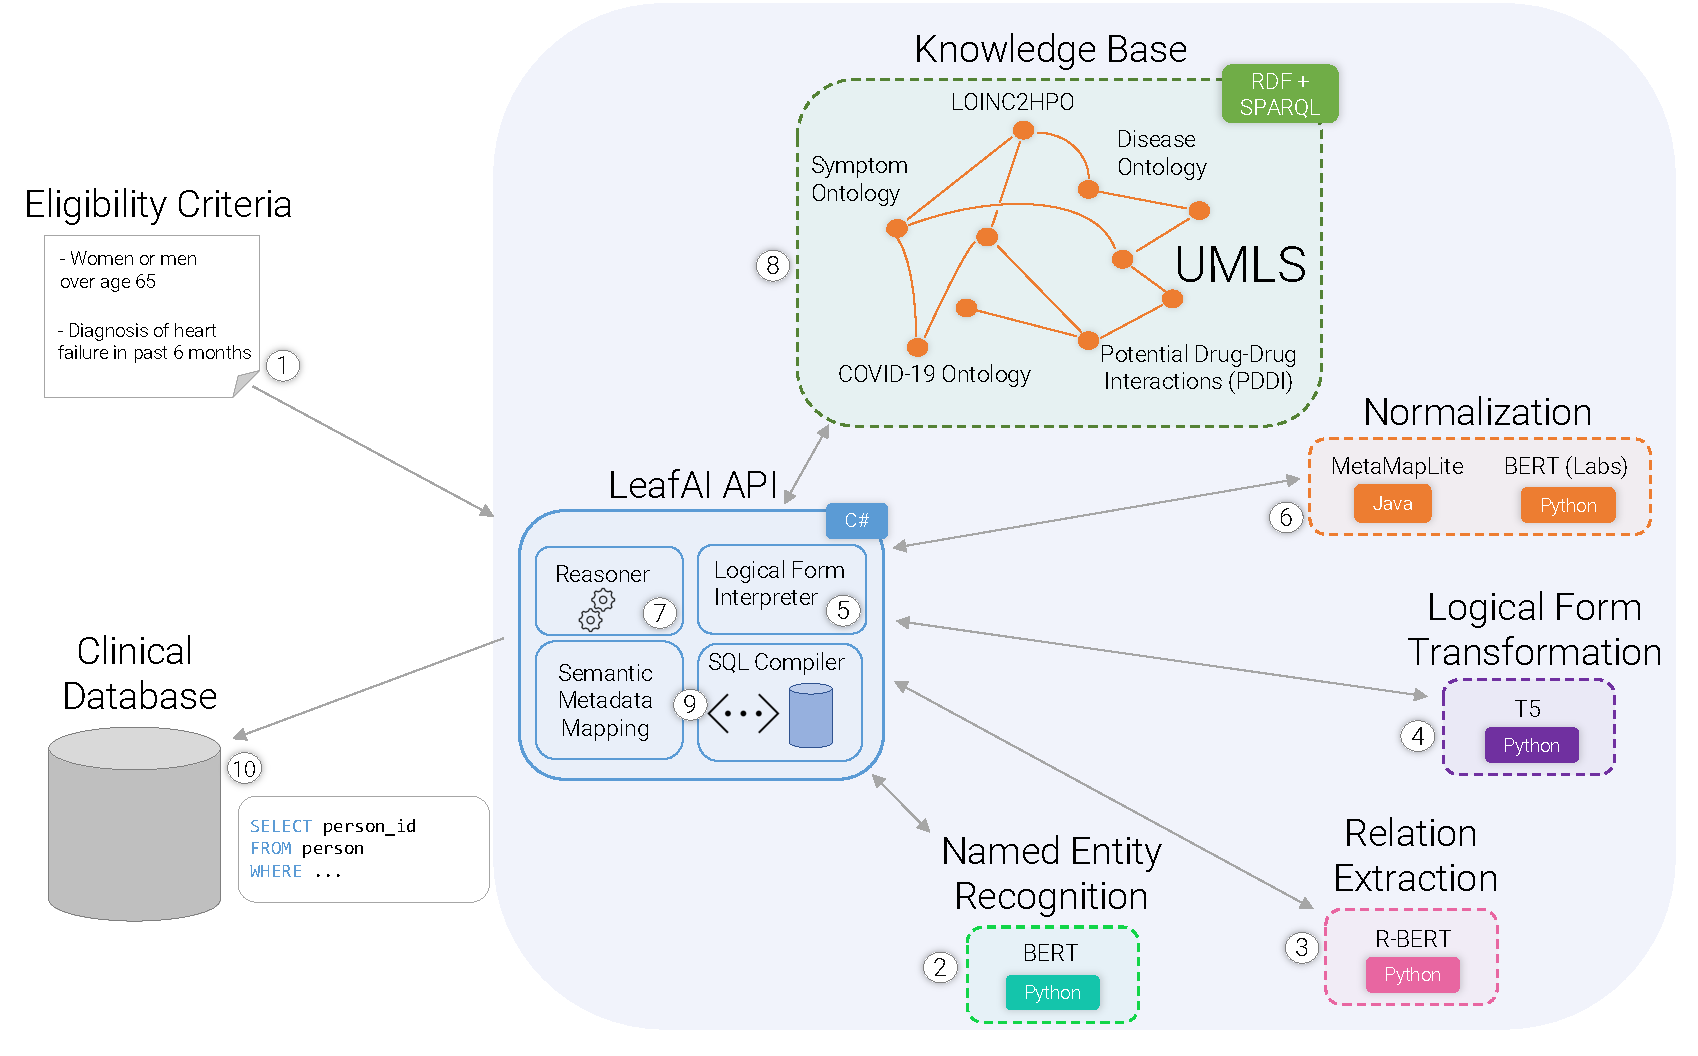
\includegraphics[scale=0.6]{figures/leafai_architecture.pdf}  
\caption{LeafAI query architecture. Inter-module communication is performed using the gRPC framework. Individual modules are deployed as Docker \cite{docker} containers and communicate solely with the central API, which orchestrates query generation and handles query generation requests.}
\label{fig_leafai_architecture}
\end{figure}

\noindent At a high level, query generation is performed in the following steps:

\begin{enumerate}
    \item{A query request is received by the API in the form of inclusion and exclusion criteria as free-text strings.}
    \item{The input texts are tokenized and named entity recognition is performed to determine spans of text representing conditions, procedures, and so on.}
    \item{Relation extraction is performed to determine relations between the entities, such as \textit{Caused-By} or \textit{Numeric-Filter}.}
    \item{The input texts are transformed by replacing spans of "raw" text with logical form names. For example, "Diagnosed with diabetes" would become "Diagnosed with cond("diabetes")." The resulting input texts are in turn transformed into an output logical representation using a Sequence to Sequence (Seq2Seq) architecture, in the form of a string.}
    \item{A logical form interpreter module implemented as a recursive descent parser \cite{johnstone1998generalised} reads the logical form string input and instantiates it as an abstract syntax tree (AST) of nested in-memory logical form objects.}
    \item{"Named" logical form objects (i.e., specified with quoted text, such as "lab("hemoglobin A1c")") are normalized into one or more corresponding UMLS concepts.}
    \item{Working recursively inside-to-outside the AST structure, each logical form object calls a \textit{Reason()} method which executes various rules depending on context.}
    \item{Each reasoning rule is performed as one or more pre-defined SPARQL queries to the knowledge base (KB), concept by concept.}
    \item{The final normalized, reasoned, logical form AST is thus a nested structure of UMLS concepts. Each AST criterion is mapped to zero or more corresponding entries in the semantic metadata mapping (SMM), which in turn lists meanings, roles, and relations of a database schema in the form of UMLS concepts.}
    \item{The final mapped AST object is transformed into a series of database queries, one per line of eligibility criteria text. The output SQL query can either be executed directly on a database or returned to the API caller.}
\end{enumerate}

\noindent Figure \ref{fig_leafai_querygen} illustrates an example of this process. In the following subsections we examine these steps in detail.

\begin{figure}[h]
  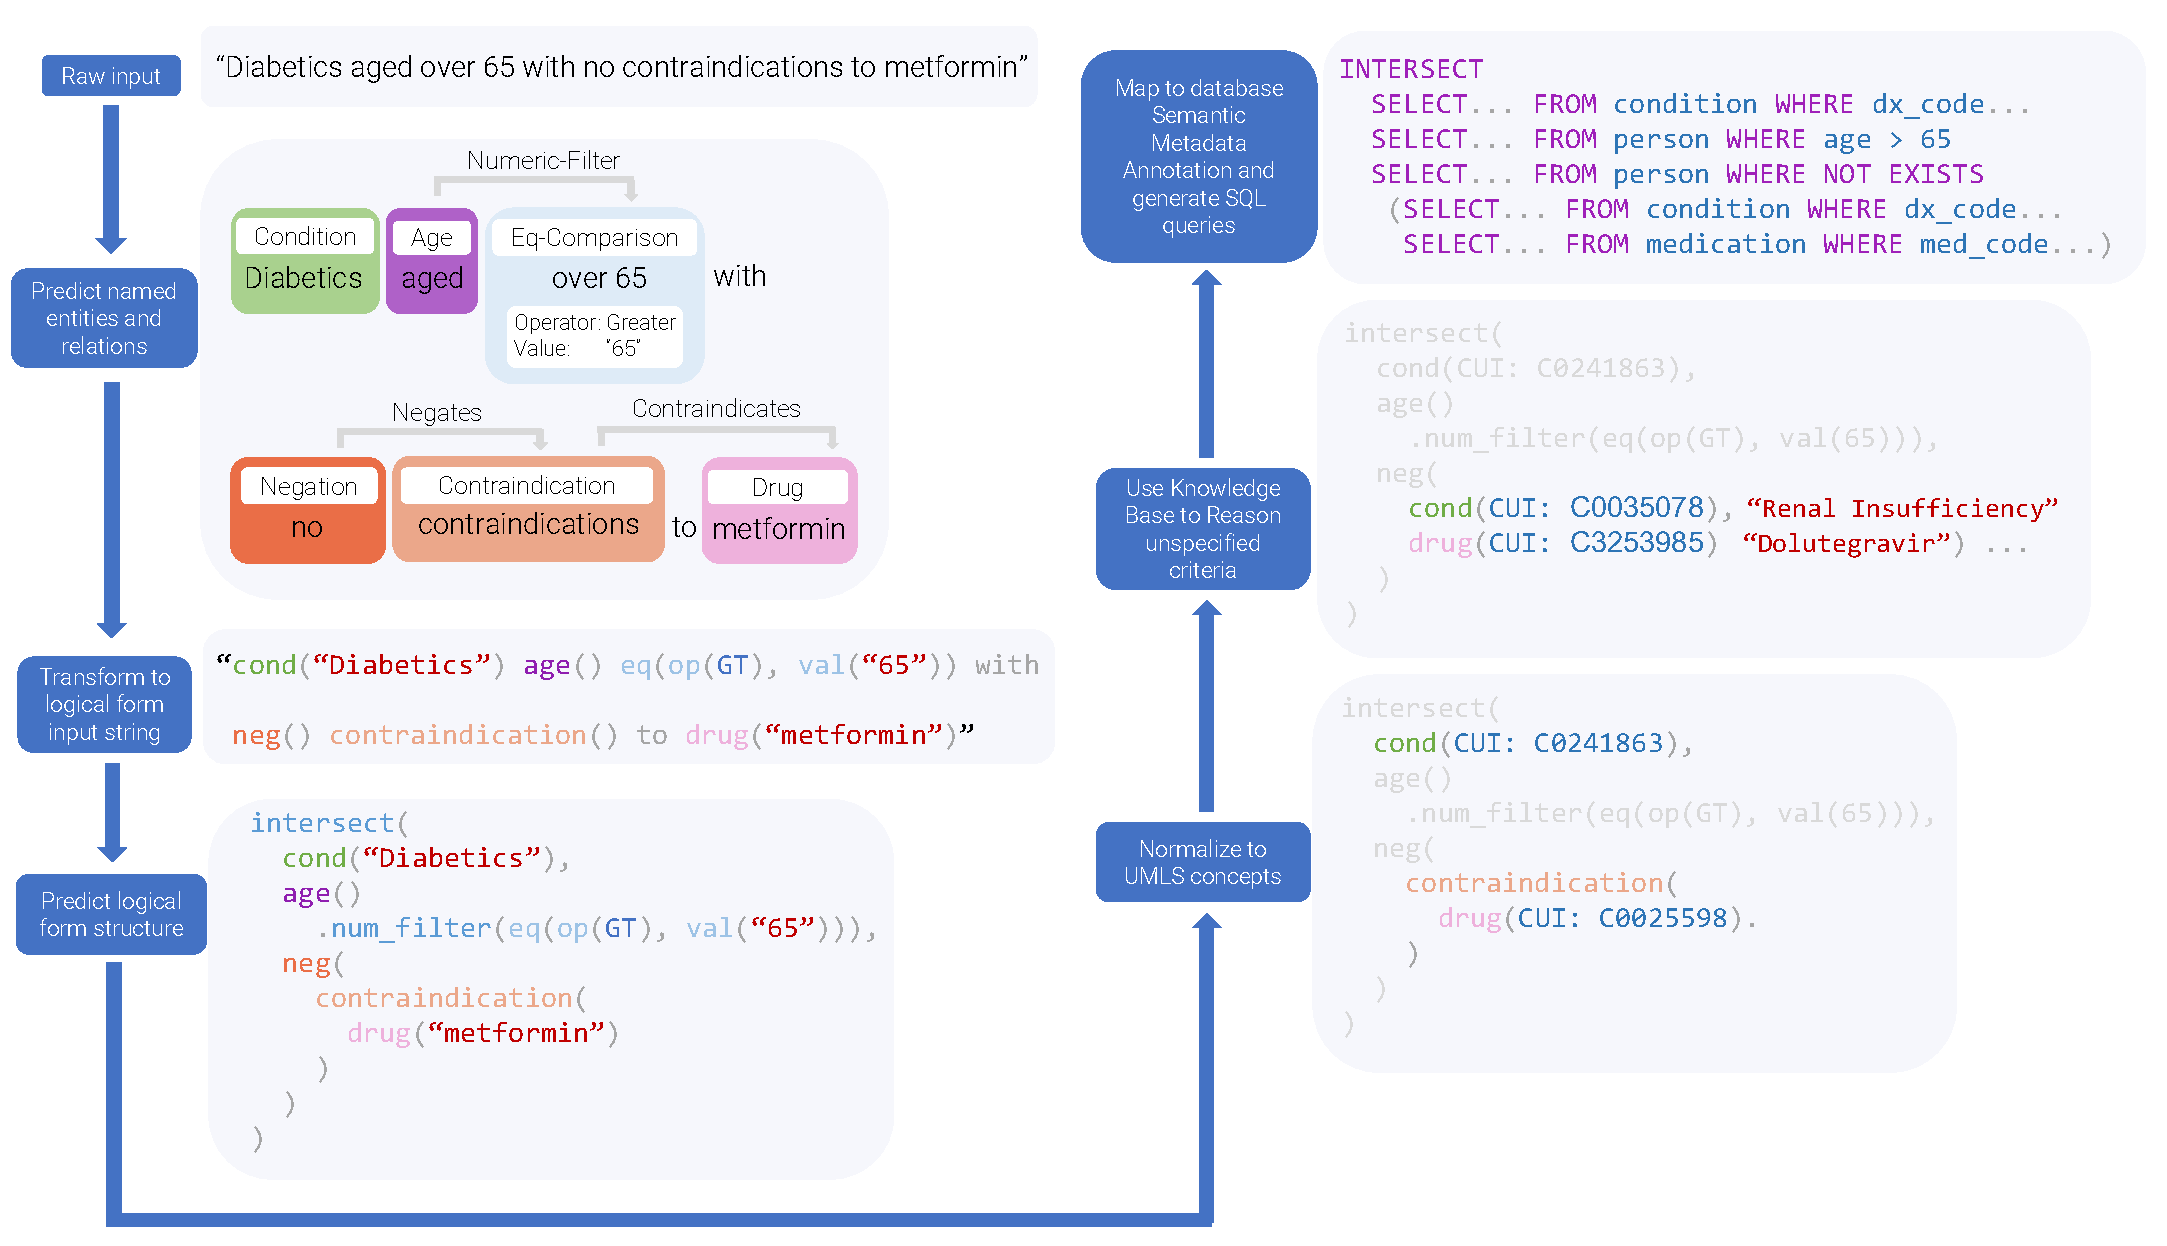
\includegraphics[scale=0.47]{figures/leafai_flow.pdf}  
\caption{LeafAI query generation processes}
\label{fig_leafai_querygen}
\end{figure}

\subsection*{Named entity recognition and relation extraction}

\noindent Named entity recognition (NER) refers to the segmentation and identification of tokens within an input sentence as "entities", such as conditions or procedures. We used the Leaf Clinical Trials (LCT) corpus \cite{dobbins2022leaf} to train two BERT-based \cite{devlin2018bert} NER extractors, one each for LCT general- and fine-grained-entities (see \cite{dobbins2022leaf} for more information on LCT entity types). Next, we perform relation extraction between named entity pairs similarly using a BERT-based model also trained on the LCT corpus.

\subsection*{Intermediate logical form transformation}

\noindent One of the core challenges of generating queries for eligibility criteria is the problem of logical representation. Works such as Criteria2Query \cite{yuan2019criteria2query} normalize and subsequently generate queries directly based on named entities and relations, which while practical, may perform poorly in cases of nested or complex logic. An alternative to this approach is to use a so-called intermediate representation (IR), which transforms the original natural language input by removing "noise" unnecessary to a given task and which more logically represents underlying semantics (see Herzig \textit{et al} \cite{herzig2021unlocking} for an examination of IR-based SQL generation approaches). Similar to earlier discussed work using Description Logics, Roberts and Demner-Fushman \cite{roberts2016annotating} proposed a representation of questions on EHR databases using a comparatively compact but flexible format using first order logic expressions, for example, representing "Is she wheezing this morning?" as

\begin{quote}
    \centering
    $\delta( \lambda x.has\_problem(x, C0043144, status) \wedge time\_within(x, \mathrm{"this\ morning"}))$
\end{quote}

\noindent This style of representation is powerfully generalizable, but also difficult to translate directly into SQL statements as multiple predicates (e.g., \textit{has\_problem} and \textit{time\_within}) may actually correspond to one or many SQL statements, depending on context, complicating direct transformation into queries.

\noindent We thus chose a similar intermediate representation (hereafter simply "logical forms") as proposed by Roberts and Demner-Fushman but more closely resembling a nested functional structure in programming languages such as Python or JavaScript and more amenable to SQL generation. A criterion such as "Diabetic women and men over age 65" would be represented by our logical forms as

\begin{quote}
$intersect( \\
    \mathrm{\ \ \ \ }cond("Diabetic"), \\
    \mathrm{\ \ \ \ }union(female(), male()),\\
    \mathrm{\ \ \ \ }age().num\_filter(eq(op(GT), val("65"))) \\
)$
\end{quote}

\noindent A description of our logical forms annotation schema, corpus, annotation process, and performance metrics can be found in Appendix A. \\

\noindent After named entity recognition and relation extraction are performed, we leverage T5 \cite{raffel2020exploring}, a state-of-the-art Seq2Seq architecture we fine-tuned for predicting logical forms. As inputs to the Seq2Seq model we use the original eligibility criteria with named entity spans replaced by logical form representations, as we found this to significantly improve performance compared to training with raw inputs without named entities. Thus the above example would be transformed to the input string

\begin{quote}
    \centering
    $\textit{"cond(“Diabetic”) female() and male() over age() eq(op(GT), val(“65”))"}$
\end{quote}

\noindent The returned logical form string is then instantiated into an abstract syntax tree (AST) of nested in-memory logical form objects using a recursive descent parser \cite{johnstone1998generalised} within the API.

\subsection*{Concept normalization}

\noindent Normalization refers to the mapping of free-text string values (e.g., "diabetes mellitus") to coded representations (e.g., UMLS, ICD-10, SNOMED, or LOINC). We normalize "named" logical forms to UMLS concepts using MetaMapLite \cite{aronson2001effective, demner2017metamap}. We consider a logical form "named" if it contains a free-text value surrounding by quotes. For example, \textit{cond()} is unnamed and refers to any condition or disease, while \textit{cond("hypertension")} is named as it refers to a specific condition. \\

\noindent Normalization using MetaMapLite can often result in high recall but low precision, as MetaMapLite has no NER component and also compares input strings to millions of concepts within the UMLS, many of which the tool cannot disambiguate from and thus returns all. To improve normalization precision, we employ two strategies. First, we compare term frequency-inverse document frequency (tf-idf) on MetaMapLite predictions, dropping UMLS concepts whose matched spans have a tf-idf score lower than that of unmatched spans in a given named entity. For example, for the string "covid-19 infection", MetaMapLite predicts both "COVID-19" (C5203670) as well as several concepts related to general infections. Using our tf-idf strategy removes the erroneous infection concepts. Next, our NER component also us to further improve precision by filtering the predicted UMLS concepts to only those of specific semantic types. For example, we limit condition concepts to only those which include semantic types of signs or symptoms, diseases or syndromes, and so on. \\

\noindent Laboratory values also present a particular challenge with MetaMapLite, as LeafAI expects predicted lab concepts to have directly associated LOINC codes, while MetaMapLite tends to normalize lab test strings to UMLS concepts of semantic type "laboratory test or finding", but which are typically distinct from concepts with direct mappings to LOINC. For example, a search for "platelet count" with MetaMapLite returns the concept "Platelet Count Measurement" (C0032181), but not the needed concept of "Platelet \# Bld Auto" (C0362994). Thus similar to Lee and Uzuner's work on normalizing medications \cite{lee2020normalizing}, we trained a separate BERT model specifically for normalization of lab tests.

\subsection*{Reasoning using an integrated knowledge base}

\noindent For reasoning and derivation of ICD-10, LOINC, and other codes for UMLS concepts, we designed a knowledge base (KB) accessible via SPARQL queries and stored as RDF triples. The core of our KB is the UMLS, derived using a variation of techniques created for ontologies in BioPortal \cite{noy2009bioportal}. To further augment the UMLS, we mapped and integrated the Disease Ontology \cite{schriml2012disease}, Symptom Ontology \cite{sayers2010database}, COVID-19 Ontology \cite{sargsyan2020covid}, Potential Drug-Drug Interactions \cite{ayvaz2015toward}, LOINC2HPO \cite{zhang2019semantic}, and the Disease-Symptom Knowledge Base \cite{wang2008automated}. We then developed SPARQL queries parameterized by UMLS concepts for various scenarios which leveraged our KB, such as contraindications to treatments, symptoms of diseases, and so on. Using LOINC2HPO mappings further allows us to infer phenotypes by lab test results rather than only ICD-10 or SNOMED codes, for example. \\

\noindent Our KB and reasoning methods also allow for powerful reasoning on eligibility criteria in a "multi-hop" fashion over several steps. For example, given the non-specific criterion "Contraindications to drugs for conditions which affect respiratory function", our KB successfully reasons that (among other results),

\begin{enumerate}
    \item \textbf{Asthma} causes changes to \textbf{respiratory function}
    \item \textbf{Methylprednisolone} can be used to treat \textbf{asthma}
    \item \textbf{Mycosis} (fungal infection) is a contraindication to \textbf{methylprednisolone}
\end{enumerate}

\noindent These features allow LeafAI to reason upon fairly complex non-specific criteria.

\subsection*{Query generation using semantic metadata mapping}

\noindent To allow for data model-agnostic query generation, we leveraged a subset of codes within the UMLS in what we define as a semantic metadata map, or SMM. An SMM is described using JSON, and includes a listing of available databases, tables, columns, and so on. Critically, these database artifacts are "tagged" using UMLS concepts. An example of this can be seen in Figure \ref{fig_leafai_smm}, which shows strategies by which a given criterion can be used to generated schema-specific queries by leveraging SMMs. In cases where the LeafAI query engine finds more than one means of querying a concept (e.g., two SQL tables for diagnosis codes), the database queries are combined in a UNION statement.

\begin{figure}[h]
  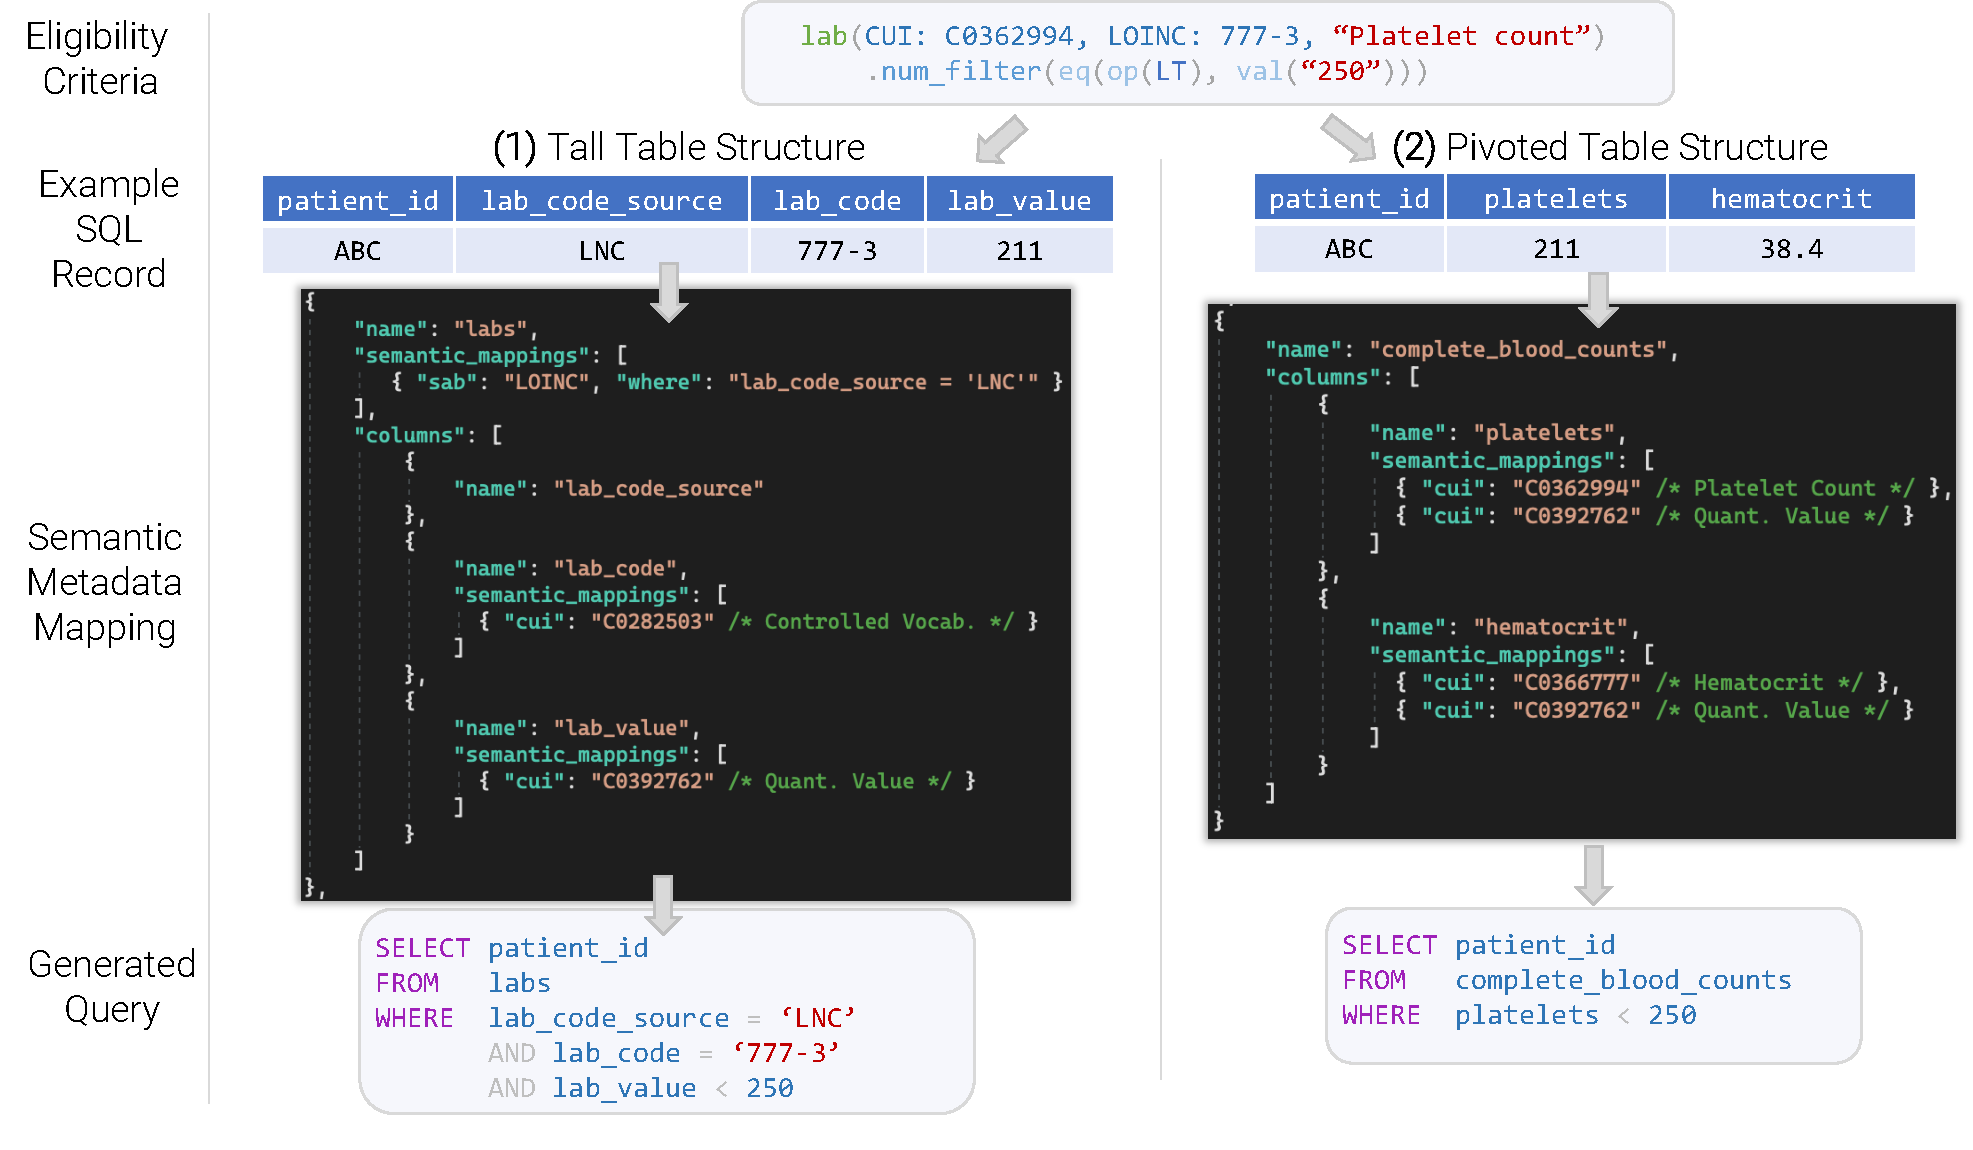
\includegraphics[scale=0.53]{figures/leafai_smm.pdf}  
\caption{The LeafAI query engine's SQL query generation process using two hypothetical database schema to generate queries for platelet counts (shown in logical form after normalization). This example illustrates the flexibility of LeafAI's semantic metadata mapping system in adapting to virtually any data model. On the left, "Tall Table Structure", platelet counts must be filtered from within a general purpose "labs" table. The LeafAI KB recognizes that labs may be stored as LOINC codes, and the corresponding SMM indicates that records in this table can be filtered to LOINC values. On the right, "Pivoted Table Structure", platelet counts are stored as a specific column in a "complete\_blood\_counts" table, and thus can be directly queried without further filtering. Additional metadata, columns, tables, types and so on needed in SMMs are omitted for brevity.}
\label{fig_leafai_smm}
\end{figure}

\subsection*{Evaluation}

\end{document}